\documentclass[12pt]{amsart}

\usepackage{graphicx}
\usepackage{amsmath}
\usepackage[pdftex]{hyperref}

\setlength{\textwidth}{6.2in}
\setlength{\textheight}{8.4in}
\setlength{\topmargin}{0.2in}
\setlength{\oddsidemargin}{0in}
\setlength{\evensidemargin}{0in}
\setlength{\headsep}{.3in}
\footskip 0.3in
\newtheorem{thm}{Theorem}
\newtheorem{lemma}[thm]{Lemma}
\newtheorem{prop}[thm]{Proposition}
\newtheorem{cor}[thm]{Corollary}
\theoremstyle{definition}
\newtheorem{defn}[thm]{Definition}
\newtheorem{example}[thm]{Example}
\newtheorem{remark}[thm]{Remark}
\newtheorem{conj}[thm]{Conjecture}

\newcommand{\cherry}[1]{\ensuremath{\langle #1 \rangle}}
\newcommand{\ignore}[1]{}
\newcommand{\half}{\frac{1}{2}}
\newcommand{\eopf}{\framebox[6.5pt]{} \vspace{0.2in}}

%------------------document begins-----------------------

\begin{document}

\title{Methods of Cufflinks}
\author{Cole Trapnell \and Lior Pachter}
%\address{}
%\email{\{whoweare\}@math.berkeley.edu}
%\dedicatory{\today}

%\thanks{Supported in part by ....}
%\subjclass{Primary 55M20; Secondary 47H10}

\maketitle
\markboth{C Trapnell and L Pachter}{Methods of Cufflinks}

This document describes the methods used in the Cufflinks RNA-Seq analysis program.
%\pagestyle{plain}
\pagenumbering{roman} \tableofcontents \listoffigures \listoftables \newpage \pagenumbering{arabic}

\section{Version 0.8.3}

\subsection{Transcript abundance estimation \label{abundances}}
\label{sec:abundances}

\subsubsection{Definitions}

A {\em transcript} is an RNA molecule that has been transcribed from DNA. A
{\em primary transcript} is an RNA molecule that has yet to undergo
modification. The {\em genomic location} of a primary transcript consists of a
pair of coordinates in the genome representing the $5'$ transcription start
site and the $3'$ polyadenylation cleavage site. We denote the set of all
transcripts in a transcriptome by $T$. We partition transcripts into {\em
transcription loci} (for simplicity we refer to these as loci) so that every
locus contains a set of transcripts all of whose genomic locations do not
overlap the genomic location of any transcript in any other locus. Formally,
we consider a maximal partition of transcripts into loci, a partition denoted
by $G$, where the genomic location of a transcript $t \in g \in G$ does not
overlap the genomic location of any transcript $u $ where $u \in h \in G$ and
$h \neq g$. We emphasize that the definition of a transcription locus is not
biological; transcripts in the same locus may be regulated via different
promoters, and may differ completely in sequence (for example if one
transcript is in the intron of another) or have different functions. The
reason for defining loci is that we will see that they are computationally
convenient.


We assume that at the time of an experiment, a transcriptome consists of an
ensemble of transcripts $T$ where the proportion of transcript $t \in T$ is
$\rho_t$, so that $\sum_{t \in T} \rho_t = 1$ and $0 \leq \rho_t \leq 1$ for
all $t \in T$. Formally, a {\em transcriptome} is a set of transcripts $T$
together with the abundances $\rho=\{ \rho_t\}_{t \in T}$. For convenience we also introduce
notation for the proportion of transcripts in each locus. We let $\sigma_g =
\sum_{t \in g} \rho_t$. Similarly, within a locus $g$, we denote the
proportion of each transcript $t \in g$ by $\tau_t = \frac{\rho_t}{\sigma_g}$.
We refer to $\rho,\sigma$ and $\tau$ as {\em transcript abundances}.


Transcripts have lengths, which we denote by $l(t)$. For a collection of transcripts $S \subset T$ in a transcriptome, we define the length of $S$ using the weighted mean:
\begin{equation}
\label{eq:effective_length}
l(S) =\frac{\sum_{t \in S} \rho_tl(t)}{\sum_{t \in S}\rho_t}.
\end{equation}
It is important to note that the length of a set of transcripts depends on their relative abundances; the reason for this will be clear later. 

One grouping of transcripts that we will focus on is the set of transcripts
within a locus that share the same transcription start site (TSS). Unlike the
concept of a locus, grouping by TSS has a biological basis. Transcripts
within such a group are by definition alternatively spliced, and if they have
different expression levels, this is most likely due to the spliceosome and
not due to differences in transcriptional regulation.

\subsubsection{A statistical model for RNA-Seq}

In order to analyze expression levels of transcripts with RNA-Seq data, it is
necessary to have a model for the (stochastic) process of sequencing. A {\em
sequencing experiment} consists of selecting a total of $M$ fragments of
transcripts uniformly at random from the transcriptome. Each fragment is
identified by sequencing from its ends, resulting in two reads called {\em
mate pairs}. The length of a fragment is a random variable, with a
distribution we will denote by $F$. That is, the probability that a fragment
has length $i$ is $F(i)$ and $\sum_{i=1}^{\infty} F(i) = 1$. In this paper we
assume that $F$ is normal, however in principle $F$ can be estimated using
data from the experiment (e.g. spike-in sequences). We decided to use
the normal approximation to $F$ (allowing for user specified
parameters of the normal distribution) in order to simplify the
requirements for running {\tt Cufflinks} at this time. 

The assumption of random
fragment selection is known to oversimplify the complexities of a sequencing
experiment, however without rigorous ways to normalize we decided to work with
the uniform at random assumption. It is easy to adapt the model to include
more complex models that address sequencing bias as RNA-Seq experiments mature
and the technologies are better understood.

The transcript abundance estimation problem in paired-end RNA-Seq is to
estimate $\rho$ given a set of transcripts $T$ and a set of reads sequenced
from the ends of fragments. In {\tt Cufflinks}, the transcripts $T$ can be
specified by the user, or alternatively $T$ can be estimated directly from the
reads. The latter problem is the transcript assembly problem which we discuss
in Section \ref{sec:assembly}. We ran {\tt Cufflinks} in the latter
``discovery'' mode where we assembled the transcripts without using the
reference annotation.

The fact that fragments have different lengths has bearing on the calculation
of the probability of selecting a fragment from a transcript. Consider a
transcript $t$ with length $l(t)$. The probability of selecting a fragment of
length $k$ from $t$ at one of the positions in $t$ assuming that it is
selected uniformly at random, is $\frac{1}{l(t)-k}$. For this reason, we will
define an adjusted length for transcripts as

\begin{equation}
\tilde{l}(t) = \sum_{i=1}^{l(t)} F(i)(l(t)-i+1).
\end{equation}
We also revisit the definition of length for a group of transcripts, and define 
\begin{equation}
\tilde{l}(S) =\frac{\sum_{t \in S} \rho_t\tilde{l}(t)}{\sum_{t \in S}\rho_t}.
\end{equation} 

It is important to note that given a read it may not be obvious from which
transcript the fragment it was sequenced from originated. The consistency of
fragments with transcripts is important and we define the {\em
fragment-transcript matrix} $A_{R,T}$ to be the $M \times |T|$ matrix with
$A(r,t)=1$ if the fragment alignment $r$ is completely contained in the
genomic interval spanned by $t$, and all the implied introns in $r$ match
introns in $t$ (in order), and with $A(r,t)=0$ otherwise. Note that the reads
in Figure 1c in the main text are colored according to the matrix $A_{R,T}$,
with each column of the matrix corresponding to one of the three colors
(yellow, blue, red) and reads colored according to the mixture of colors
corresponding to the transcripts their fragments are contained in.

Even given the read
alignment to a reference genome, it may not be obvious what the length of the
fragment was. Formally, in the case that $A_{R,T}(r,t)=1$ we denote by $I_t(r)$ the fragment length from within
a transcript $t$ implied by the (presumably unique) sequences corresponding to
the mate pairs of a fragment $r$. If $A_{R,T}(r,t)=0$ then $I_t(r)$ is set to be
infinite and $F(I_t(r)) = 0$. 

Given a set of reads, we assume that we can identify for each of them the set
of transcripts with which the fragments the reads belonged to are consistent. The
rationale for this assumption is the following: we map the reads to a
reference genome, and we assume that the read lengths are sufficiently long so
that every mate-pair can be uniquely mapped to the genome. We refer to this
mapping as the {\em fragment alignment}. We also assume that we know all the
possible transcripts and their alignments to the genome. Therefore, we can
identify for each read the possible transcripts from which the fragment it
belonged to originated.

\begin{figure}[!ht] 
    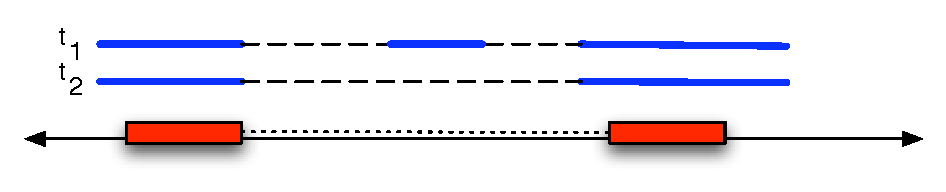
\includegraphics[scale=0.8]{pdfs/implied_length}
    \caption[Implied length of a fragment alignment]{Alignments of reads to the genome (rectangles) may be consistent with multiple transcripts (in this case both $t_1$ and $t_2$). The transcripts $t_1$ and $t_2$ differ by an internal exon; introns are indicated by long dashed lines. If we denote the fragment alignment by $r$, this means that $A_{R,T}(r,t_1)=1$ and $A_{R,T}(r,t_2)=1$. It is apparent that the implied length $I_{t_1}(r) > I_{t_2}(r)$ due to the presence of the extra internal exon in $t_1$. }
\end{figure}

We are now ready to write down the likelihood equation for the model. We will
write $L(\rho|R)$ for the likelihood of a set of fragment alignments $R$
constructed from $M$ reads. The notation $Pr(trans. = t)$ means ``the
probability that a fragment selected at random originates from transcript $t$''.

\begin{eqnarray}
& & L(\rho|R) = \prod_{r \in R} Pr(rd.\ aln. =r)\\
&  = & \prod_{r \in R} \sum_{t \in T} Pr(rd.\ aln. =r|trans. =t)Pr(trans. =t)\\
& = & \prod_{r \in R} \sum_{t \in T} \frac{\rho_t\tilde{l}(t)}{\sum_{u \in T}\rho_u\tilde{l}(u)} Pr(rd.\ aln. = r|trans. =t)\\ 
& = & \prod_{r \in R} \sum_{t \in T}\frac{\rho_t\tilde{l}(t)}{\sum_{u \in T}\rho_u\tilde{l}(u)} \left(\frac{F(I_t(r))}{l(t)-I_t(r)+1}\right) \\ \label{eq:likerho}
& = &  \prod_{r \in R} \sum_{t \in T} \alpha_t\left(\frac{F(I_t(r))}{l(t)-I_t(r)+1}\right),
\end{eqnarray}
where 
\begin{equation}
\alpha_t = \frac{\rho_t\tilde{l}(t)}{\sum_{u \in T}\rho_u\tilde{l}(u)}.
\end{equation}

Observe that $\alpha_t$ is exactly the probability that a fragment selected at
random comes from transcript $t$, and we have that $\sum_{t \in T}\alpha_t =
1$. In light of the probabilistic meaning of the $\alpha=\{\alpha_t\}_{t \in T}$, we refer to them as
{\em fragment abundances}.

It is evident that the likelihood function is that of a linear model
and  that the likelihood function is
concave (Proposition \ref{prop:linearmodel}) so a numerical method can be used
to find the $\alpha$. It is then possible, in principle, to recover the $\rho$
using Lemma \ref{lemma:readstoprobs}. However the number of parameters is in the tens of
thousands, and in practice this form of the likelihood function is unwieldy.
Instead, we re-write the likelihood utilizing the fact that transcripts in
distinct loci do not overlap in genomic location.

We first calculate the  probability that a fragment originates from a transcript within a given locus $g$:
\begin{eqnarray}
\beta_g & := &  \sum_{t \in g} \alpha_t\\
& = & \frac{\sum_{t \in g} \rho_t \tilde{l}(t)}{\sum_{u \in T} \rho_u \tilde{l}(u)}\\
& = & \frac{\sum_{t \in g} \sigma_g\tau_t \tilde{l}(t)}{\sum_{h \in G} \sum_{u \in h} \sigma_h\tau_u \tilde{l}(u)}\\
& = & \frac{\sigma_g\sum_{t \in g} \tau_t \tilde{l}(t)}{\sum_{h \in G} \sigma_h \sum_{u \in h} \tau_u \tilde{l}(u)}\\
 & = &  \frac{\sigma_g \tilde{l}(g)}{\sum_{h \in G} \sigma_h \tilde{l}(h)}. 
\end{eqnarray}
Recall that $\sigma_g = \sum_{t \in g} \rho_t$ and that $\tau_t = \frac{\rho_t}{\sigma_g}$ for a locus $g$. 

Similarly, the probability of selecting a fragment from a single transcript $t$ conditioned on selecting a transcript from the locus $g$ in which $t$ is contained is
\begin{equation}
\label{eq:gammatau}
\gamma_t = \frac{\tau_t \tilde{l}(t)}{\sum_{u \in g} \tau_u \tilde{l}(u)}. 
\end{equation}
The parameters $\gamma=\{\gamma_t\}_{t \in g}$ are conditional fragment abundances, and they are the parameters we estimate from the data in the next Section. Note that for a transcript $t \in g$, $\alpha_t = \beta_g \cdot \gamma_t$ and it is easy to convert between fragment abundances and transcript abundances using Lemma \ref{lemma:readstoprobs}.

We denote the fragment counts by $X$; specifically, we denote the number of
alignments in locus $g$ by $X_g$. Note that $\sum_{g \in G} X_g = M$. We also
use the notation $g_r$ to denote the (unique) locus from which a read
alignment $r$ can be obtained.

The likelihood function is given by
\begin{eqnarray}
& & L(\rho|R) = \prod_{r \in R} Pr(rd.\ aln. =r)\\
&  = & \prod_{r \in R} \sum_{g \in G} Pr(rd.\ aln. =r|locus=g)Pr(locus=g)\\
& = & \prod_{r \in R} \frac{\sigma_{g_{r}}\tilde{l}(g_{r})}{\sum_{g \in G} \sigma_g\tilde{l}(g)} Pr(rd.\ aln. =r|locus=g_r)\\
& = & \prod_{r \in R}  \beta_{g_r}
\sum_{t \in g_r}Pr(rd.\ aln. =r|locus=g_{r},trans. = t)Pr(trans. =t|locus=g_r)\\
& = & \prod_{r \in R} \beta_{g_r}
\sum_{t \in g_r} \frac{\tau_t\tilde{l}(t)}{\sum_{u \in g_r}\tau_u \tilde{l}(u)} Pr(rd.\ aln. =r|locus=g_{r},trans. = t)\\ 
& = & \left( \prod_{r \in R} \beta_{g_r} \right) \left( \prod_{r \in R} \sum_{t \in g} \gamma_t \cdot
Pr(rd.\ aln. =r|locus=g_r,trans. =t) \right)\\
& = & \left( \prod_{r \in R}  \beta_{g_r} \right) \left( \prod_{r \in R} \sum_{t \in g}  \gamma_t\cdot  \frac{F(I_t(r))}{l(t)-I_t(r)+1}\right)\\
& = & \left( \prod_{g \in G}  \beta_g^{X_{g}} \right) \left( \prod_{g \in G} \left( \prod_{r \in R:r \in g} \sum_{t \in g}  \gamma_t \cdot
\frac{F(I_t(r))}{l(t)-I_t(r)+1}\right) \right). \label{eq:likebest}
\end{eqnarray}

Explicitly, in terms of the parameters $\rho$, Equation (\ref{eq:likebest})
simplifies to Equation (\ref{eq:likerho}) but we will see in the next section
how the maximum likelihood estimates $\hat{\rho}$ are most conveniently
obtained by first finding $\hat{\beta}$ and $\hat{\gamma}$ using Equation
(\ref{eq:likebest}).

We note that it is biologically meaningful to include prior distributions on
$\sigma$ and $\tau$ that reflect the inherent stochasticity and resulting
variability of transcription in a cell. This will be an interesting direction
for further research as more RNA-Seq data (with replicates) becomes available
allowing for the determination of biologically meaningful priors. In
particular, it seems plausible that specific isoform abundances may vary
considerably and randomly within cells from a single tissue and that this may
be important in studying differential splicing. We mention to this to clarify
that in this paper, the confidence intervals we report represent the
variability in the maximum likelihood estimates $\hat{\sigma}_j$ and
$\hat{\tau}^k_j$, and are not the variances of prior distributions.


\subsubsection{Estimation of parameters}

We begin with a discussion of identifiability of our
model. Identifiability refers to the injectivity of the model, i.e.,
\begin{equation}
\mbox{if } Pr_{\rho_1}(r) = Pr_{\rho_2}(r) \  \forall r \in R, \ \mbox{ then } \rho_1 = \rho_2.
\end{equation}


The identifiability of RNA-Seq models was discussed in
\cite{Hiller2009}, where a standard analysis for linear models is
applied to RNA-Seq (for another related biological example, see \cite{Pe'er2004} which discusses
identifiability of haplotypes in mixed populations from genotype data).
The results in these papers apply to our model. For completeness we review the conditions for
identifiability. Recall that $A_{R,T}$ is the fragment-transcript matrix that specifies which transcripts each fragment is compatible with. The following theorem provides a simple characterization of identifiability:

\begin{thm}
The RNA-Seq model is identifiable iff $A_{R,T}$ is full rank.
\end{thm}

Therefore, for a given set of transcripts and a read set $R$, we can
test whether the model is identifiable using elementary linear
algebra. For the results in this paper, when estimating expression
with given annotations, when the model was not identifiable we picked {\em a} maximum likelihood solution,
although in principle it is possible to bound the total expression of
the locus and/or report identifiability problems to the user. 

Returning to the likelihood function
\begin{equation}
\left( \prod_{g \in G}  \beta_g^{X_{g}} \right) \left( \prod_{g \in G} \left( \prod_{r \in R:r \in g} \sum_{t \in g}  \gamma_t \cdot
\frac{F(I_t(r))}{l(t)-I_t(r)+1}\right) \right),
\end{equation}
we note that both the $\beta$ and $\gamma$ parameters depend on the $\rho$ parameters. However, we will see that if we maximize the $\beta$ separately from the $\gamma$, and also each of the sets $\{\gamma_t:t \in g\}$ separately, then it is always possible to find $\rho$ that match both the maximal $\beta$ and $\gamma$. In other words, 
the problem of finding $\hat{\rho}$ is equivalent
to finding $\hat{\beta}$ that maximizes 
$ \prod_{g \in G} \beta_g^{X_g}$
and separately, for each locus $g$, the $\hat{\gamma}_t$ that maximize
\begin{equation}
\prod_{r \in R:r \in g} \sum_{t \in g}  \gamma_t
\frac{F(I_t(r))}{l(t)-I_t(r)+1}.
\end{equation}

We begin by solving for the $\hat{\beta}$ and $\hat{\gamma}$ and the variances
of the maximum likelihood estimates, and then explain how these are used to
report expression levels.

We can solve for the $\hat{\gamma}$ using the fact that the model is linear.
That is, the probability of each individual read is linear in the read
abundances $\gamma_t$. It is a standard result in statistics (see, e.g.,
Proposition 1.4 in \cite{ASCB2005}) that the log likelihood function of a
linear model is concave. Thus, a hill climbing method can be used to find the
$\hat{\gamma}$. We used the EM algorithm for this purpose.

Rather than using the direct ML estimates, we obtained a regularized
estimate by importance sampling from the posterior distribution with a
proposal distribution we explain below. The samples were also used to estimate
variances for our estimates. 

It follows from standard MLE asymptotic
theory that the $\hat{\gamma}$ are asymptotically multivariate normal with
variance-covariance matrix given by the inverse of the observed Fisher
information matrix. This matrix is defined as follows:

\begin{defn}[Observed Fisher information matrix]
The observed Fisher information matrix is the negative of the Hessian of the log likelihood function evaluated at the maximum likelihood estimate. That is, for parameters $\Theta=(\theta_1,\ldots,\theta_n)$, the $n \times n$ matrix is
\begin{eqnarray}
\mathcal{F}_{k,l}(\hat{\Theta}) & = & - \frac{\partial^2 log(\mathcal{L}(\Theta|R))}{\partial \theta_k \theta_l} |_{\theta=\hat{\theta}}.
\end{eqnarray}
\end{defn}
In our case, considering a single locus $g$, the parameters are $\Theta = (\gamma_{t_1},\ldots,\gamma_{t_{|g|}})$, and as expected from Proposition \ref{prop:linearmodel}:
\begin{eqnarray}
\label{eq:Fisher}
\mathcal{F}_{t_k,t_l}(\hat{\Theta}) & = & \sum_{r \in R:r \in g}
\left[ \frac{1}{\left( \sum_{h \in g}  \hat{\gamma}_h \frac{F(I_h(r))}{l(h) - I_h(r)+1} \right)^2} \frac{F(I_{t_k}(r)) F(I_{t_l}(r)) }{(l(t_k)-I_{t_k}+1)(l(t_l)-I_{t_l}+1)} \right].
\end{eqnarray}


Because some of the transcript abundances may be close to zero, we
adopted the
Bayesian approach of \cite{Jiang2009} and instead sampled from the
joint posterior distribution of $\Theta$ using the proposal
distribution consisting of the multivariate normal with mean
given by the MLE, and variance-covariance matrix given by the inverse of
(\ref{eq:Fisher}). If the Observed Fisher Information Matrix is
singular then the user is warned and the confidence intervals of all
transcripts are set to $[0,1]$ (meaning that there is no information
about relative abundances).

The method used for sampling was importance sampling. The samples were used to obtain a maximum-a-posterior estimate for
$\hat{\gamma}_t$ for each $t$ and for the variance-covariance matrix which we
denote by $\Psi^g$ (where $g \in G$ denotes the locus). Note that $\Psi^g$ is
a $|g| \times |g|$ matrix. The covariance between $\hat{\gamma}_{t_k}$ and
$\hat{\gamma}_{t_l}$ for $t_k,t_l \in g$ is given by $\Psi^g_{t_k,t_l}$.

Turning to the maximum likelihood estimates $\hat{\beta}$, we use the fact that the model is the log-linear. Therefore, 
\begin{equation}
\label{eq:sigmahat}
\hat{\beta_g} = \frac{X_{g}}{M}.
\end{equation}

Viewed as a random variable, the counts $X_{g}$ are approximately Poisson and therefore the variance of the MLE $\hat{\beta}_g$ is approximately $X_{g}$. We note that for the tests in this paper we directly used the total counts $M$ and the proportional counts $X_g$, however it is easy to incorporate recent suggestions for total count normalization, such as \cite{Bullard2010} into {\tt Cufflinks}.

The favored units for reporting expression in RNA-Seq studies to date is not
using the transcript abundances directly, but rather using a measure
abbreviated as FPKM, which means ``expected number of fragments per kilobase
of transcript sequence per millions base pairs sequenced''. These units are
equivalent to measuring transcript abundances (multiplied by a scalar). The
computational advantage of FPKM, is that the normalization constants
conveniently simplify some of the formulas for the variances of transcript
abundance estimates.

For example, the abundance of a transcript $t \in g$ in FPKM units is
\begin{equation}
\label{eq:FPKM1}
 \frac{10^6 \cdot 10^3 \cdot \alpha_t}{\tilde{l}(t)} =  \frac{10^6 \cdot 10^3 \cdot \beta_g \cdot \gamma_t}{\tilde{l}(t)}.
\end{equation}

Equation (\ref{eq:FPKM1}) makes it clear that although the abundance of each
transcript $t \in g$ in FPKM units is proportional to the transcript abundance
$\rho_t$ it is given in terms of the read abundances $\beta_g$ and $\gamma_t$
which are the parameters estimated from the likelihood function.

The maximum likelihood estimates of $\beta_g$ and $\gamma_t$ are random
variables, and we denote their scaled product (in FPKM units) by $A_t$. That
is $Pr(A_t = a)$ is the probability that for a random set of fragment alignments
from a sequencing experiment, the maximum likelihood estimate of the
transcript abundance for $t$ in FPKM units is $a$.

Using the fact that the expectation of a product of independent random
variables is the product of the expectations, for a transcript $t \in g$ we
have
\begin{equation}
E[A_t] = \frac{10^9X_{g}\hat{\gamma}_t}{\tilde{l}(t)M}.
\end{equation}

Given the variance estimates for the $\hat{\gamma}_t$ we turn to the problem of estimating $Var[A_t]$ for a transcript $t \in g$. We use Lemma \ref{lemma:varproduct} to obtain
\begin{eqnarray}
Var[A_t]& =  & \left(\frac{10^9}{\tilde{l}(t)M}\right)^2 \left( \Psi^g_{t,t}X_{g} + \Psi^g_{t,t}X^2_{g} + (\hat{\gamma}_t)^2 X_{g} \right)\\
& = & X_{g}\left(\frac{10^9}{\tilde{l}(t)M)}\right)^2  \left( \Psi^g_{t,t}(1+X_{g}) + (\hat{\gamma}_t)^2\right).
\end{eqnarray}

This variance calculation can be used to estimate a confidence interval by
utilizing the fact \cite{Aroian1978} that when the expectation divided by the
standard deviation of at least one of two random variables is large, their
product is approximately normal.

Next we turn to the problem of estimating expression levels (and variances of
these estimates) for groups of transcripts. Let $S \subset T$ be a group of
transcripts located in a single locus $g$, e.g. a collection of transcripts
sharing a common TSS.

The analogy of Equation (\ref{eq:FPKM1}) for the FPKM of the group is
\begin{eqnarray}
\label{eq:grouphard}
& & \frac{10^6 \cdot 10^3 \cdot \beta_g \cdot \left( \sum_{t \in S} \gamma_t\right)}{\tilde{l}(S)}\\ 
& = & 10^6 \cdot 10^3 \cdot \beta_g \cdot \sum_{t \in S} \frac{\gamma_t}{\tilde{l}(t)}. \label{eq:groupeasy}
\end{eqnarray}

As before, we denote by $B_S$ the random variables for which $Pr(B_S = b)$ is
the probability that for a random set of fragment alignments from a sequencing
experiment, the maximum likelihood estimate of the transcript abundance for
all the transcripts in $S$ in FPKM units is $b$. We note that the $B_S$ are
products and sums of random variables (Equation (\ref{eq:groupeasy})). This
makes Equation (\ref{eq:groupeasy})  more useful than the
equivalent unsimplified Equation (\ref{eq:grouphard}), especially because
$\tilde{l}(S)$ is, in general, a ratio of two random variables.

We again use the fact that the expectation of independent random variables is
the product of the expectation, in addition to the fact that expectation is a
linear operator to conclude that for a group of transcripts $S$,

\begin{equation}
\label{eq:expectTSS}
E[B_S] = \frac{10^9 \cdot X_g \cdot \sum_{t \in S} \frac{\hat{\gamma}_t}{\tilde{l}(t)}}{M}.
\end{equation}
In order to compute the variance of $B_S$, we first note that 
\begin{equation}
Var\left[\sum_{t \in S} \frac{\hat{\gamma}_t}{\tilde{l}(t)}\right] = \sum_{t \in S}\frac{1}{\tilde{l}(t)^2}\Psi^g_{t,t} + \sum_{t,u \in S} \frac{1}{\tilde{l}(t)\tilde{l}(u)} \Psi^g_{t,u}.
\end{equation}
Therefore,
\begin{eqnarray}
& & \quad Var[B_S] \quad = \quad \nonumber \\ 
& &  X_g\left(\frac{10^9}{M}\right)^2\left( \left(1+X_g\right) \left(\sum_{t \in S}\frac{1}{\tilde{l}(t)^2}\Psi^g_{t,t} + \sum_{t,u \in S} \frac{1}{\tilde{l}(t)\tilde{l}(u)} \Psi^g_{t,u}\right) + \left( \sum_{t \in S} \frac{\hat{\gamma}_t}{\tilde{l}(t)} \right)^2 \right). \label{eq:varTSS}
\end{eqnarray}

We can again estimate a confidence interval by utilizing the fact that $B_S$
is approximately normal \cite{Aroian1978}.

\subsection{Transcript assembly}
\label{sec:assembly}
\subsubsection{Overview}

{\tt Cufflinks} takes as input alignments of RNA-Seq fragments to a reference
genome and, in the absence of an (optional) user provided annotation, initially assembles transcripts from the alignments. Transcripts in
each of the loci are assembled independently. The assembly algorithm
is designed to aim for the following:
\begin{enumerate}
\item Every fragment is consistent with at least one assembled
  transcript.
\item Every transcript is tiled by reads.
\item The number of transcripts is the smallest required to satisfy requirement (1).
\item The resulting RNA-Seq models (in the sense of Section \ref{sec:abundances}) are identifiable.
\end{enumerate}
In other words, we seek an assembly that parsimoniously “explains” the fragments from the RNA-Seq experiment; every
fragment in the experiment (except those filtered out during a preliminary
error-control step) should have come from a {\tt Cufflinks} transcript, and
{\tt Cufflinks} should produce as few transcripts as possible with that property.
Thus, {\tt Cufflinks} seeks to optimize the criterion suggested in \cite{Xing2004},
however, unlike the method in that paper, {\tt Cufflinks} leverages Dilworth's
Theorem \cite{Dilworth1950} to solve the problem by reducing it
to a matching problem via the equivalence of Dilworth's and K\"{o}nig's theorems (Theorem \ref{thm:dilko} in Appendix A). Our approach to isoform reconstruction is inspired by a similar approach used for haplotype reconstruction from HIV quasi-species \cite{Eriksson2008}.

\subsection{A partial order on fragment alignments}

The {\tt Cufflinks} program loads a set of alignments in SAM format sorted by reference
position and assembles non-overlapping sets of alignments independently. After
filtering out any erroneous spliced alignments or reads from incompletely
spliced RNAs, {\tt Cufflinks} constructs a partial order (Definition \ref{def:po}), or equivalently a directed acyclic graph (DAG), with
one node for each fragment that in turn consists of an aligned pair of mated reads. First, we note that fragment alignments are of two types: those where reads align in their entirety to the genome, and reads which have a split alignment (due to an implied intron). 

In the case of single reads, the partial order can be simply
constructed by checking the reads for {\em compatibility}. Two reads
are {\em compatible} if their overlap contains the exact same implied
introns (or none). If two reads are not compatible they are {\em
  incompatible}. The reads can be partially ordered by defining, for
two reads $x,y$, that $x\leq y$ if the starting coordinate of $x$ is
at or before the starting coordinate of $y$, and if they are
compatible.

In the case of paired-end RNA-Seq the situation is more complicated
because the unknown sequence between mate pairs. To understand this,
we first note that pairs of fragments can still be determined to be
incompatible if they cannot have originated from the same
transcript. As with single reads, this happens when there is
disagreement on implied introns in the overlap. However compatibility
is more subtle. We would like to define a pair of fragments $x,y$ to
be compatible if they do not overlap, or if every implied intron in one fragment overlaps an identical implied intron in the other fragment. 

However it is important to note that it may be impossible to determine
the compatibility (as defined above) or incompatibility of a pair of fragments. For example, an unknown region internal to a fragment may overlap two different introns (that are incompatible with each other). The fragment may be compatible with one of the introns (and the fragment from which it originates) in which case it is incompatible with the other. Since the opposite situation is also feasible, compatibility (or incompatibility) cannot be assigned. Fragments for which the compatibility/incompatibility cannot be determined with respect to every other fragment are called {\em uncertain}. Finally, two fragments are called {\em nested} if one is contained within the other.


\begin{figure}[h] 
    \includegraphics[scale=0.5]{pdfs/compatibility.pdf}
    \caption[Compatibility and incompatibility of
    fragments]{Compatibility and incompatibility of
      fragments. End-reads are solid lines, unknown sequences within
      fragments are shown by dotted lines and implied introns are
      dashed lines. The reads in (a) are compatible, whereas the
      fragments in (b) are incompatible. The fragments in (c) are
      nested. Fragment $x_4$ in (d) is uncertain, because $y_4$ and
      $y_5$ are incompatible with each other.}
\end{figure}

Before constructing a partial order, fragments are extended to include
their nested fragments and uncertain fragments are discarded. These discarded fragments
are used in the abundance estimation. In theory, this may result in
suboptimal (i.e. non-minimal assemblies) but we determined empirically
that after assembly uncertain fragments are almost always consistent
with one of the transcripts. When they are not, there was no
completely tiled transcript that contained them. Thus, we employ a
heuristic that substantially speeds up the program, and that works
in practice.

A partial order $P$ is then constructed from the remaining fragments
by declaring that $x \leq y$ whenever the fragment corresponding to
$x$ begins at, or before, the location of the fragment corresponding
to $y$ and $x$ and $y$ are compatible. In what follows we identify $P$
with its Hasse diagram (or covering relation), equivalently a directed
acyclic graph (DAG) that is the transitive reduction. 

\begin{prop}
$P$ is a partial order.
\end{prop}
{\bf Proof}: The fragments can be totally ordered according to the locations where they begin. It therefore suffices to check that if $x,y,z$ are fragments with $x$ compatible with $y$ and $y$ compatible with $z$ then $x$ is compatible with $z$. Since $x$ is not uncertain, it must be either compatible or incompatible with $z$. The latter case can occur only if $x$ and/or $z$ contain implied introns that overlap and are not identical. Since $y$ is not nested within $z$ and $x$ is not nested within $y$, it must be that $y$ contains an implied intron that is not identical with an implied intron in either $x$ or $z$. Therefore $y$ cannot be compatible with both $x$ and $z$. \qed

\subsection{Assembling a parsimonious set of transcripts}

In order to assemble a set of transcripts, {\tt Cufflinks} finds a
(minimum) partition of $P$ into chains (see Definition
\ref{def:po}). A partition of $P$ into chains yields an assembly
because every chain is a totally ordered set of compatible fragments
$x_1,\ldots,x_l$ and therefore there is a set of overlapping fragments
that connects them. By Dilworth's theorem (Theorem \ref{thm:Dilworth}), the problem of finding a minimum partition $P$ into chains is equivalent to finding a maximum antichain in $P$ (an antichain is a set of mutually incompatible fragments). Subsequently, by Theorem \ref{thm:dilko}, the problem of finding a maximum antichain in $P$ can be reduced to finding a maximum matching in a certain bipartite graph that emerges naturally in deducing Dilworth's theorem from K\"{o}nig's theorem \ref{thm:konig}. 
We call the key bipartite graph the ``reachability'' graph. It is the transitive closure of the DAG, i.e. it is the graph 
where each fragment $x$ has nodes $L_x$ and $R_x$ in the left and
right partitions of the reachability graph respectively, and where there is an edge between $L_x$ and $R_y$ when $x \leq y$ in $P$. The maximum matching problem is a classic problem that admits a polynomial time algorithm. The Hopcroft-Karp algorithm \cite{Hopcroft1973} has a run time of $O(\sqrt{V}E)$ where in our case $V$ is the number of fragments and $E$ depends on the extent of overlap, but is bounded by a constant times the coverage depth. We note that our parsimony approach to assembly therefore has a better complexity than the $O(V^3)$ PASA algorithm \cite{Haas2003}. 

The minimum cardinality chain decomposition computed using the approach above may not be unique.
For example, a locus may contain two putative distinct initial exons (defined by overlapping incompatible fragments), and one
of two distinct terminal and a constitutive exon in between that is longer than any
read or insert in the RNA-Seq experiment. In such a case, the parsimonious assembly will consist of two transcripts, but there are four possible solutions that are all minimal. In order to ``phase'' distant exons, we leverage the fact that abundance inhomogeneities can link distant exons via their coverage. We therefore weight the edges of the bipartite reachability graph based on the percent-spliced-in metric introduced by
Wang \emph{et al.} in \cite{Wang2008}. In our setting, the percent-spliced-in
$\psi_x$ for an alignment $x$ is computed by counting the alignments
overlapping $x$ in the genome that are compatible with $x$ and dividing by the
total number of alignments that overlap $x$, and normalizing for the length of
the $x$. The cost $C(y,z)$ assigned to an edge between alignments $y$ and $z$ reflects
the belief that they originate from different transcripts:


\begin{equation}
    C(y,z) = -\log(1 - |\psi_y - \psi_z|).
    \label{eq:match_cost} 
\end{equation}

Rather than using the Hopcroft-Karp algorithm,  a modified version of the {\tt
LEMON} \cite{LEMON} and {\tt Boost} \cite{Boost} graph libraries are used to
compute a {\em min-cost} maximum cardinality matching on the bipartite compatibility
graph. Even with the presence of weighted edges, our algorithm is
very fast. The best known algorithm for weighted matching is $O(V^2logV+VE)$.

Because we isolated total RNA, we
expected that a small fraction of our reads would come from the intronic
regions of incompletely processed primary transcripts. Moreover, transcribed
repetitive elements and low-complexity sequence result in ``shadow''
transfrags that we wished to discard as artifacts. Thus, {\tt Cufflinks}
heuristically identifies artifact transfrags and suppresses them in its
output. We also filter extremely low-abundance minor isoforms of alternatively
spliced genes, using the model described in Section \ref {abundances} as a
means of reducing the variance of estimates for more abundant transcripts. A
transcript $x$ meeting any of the following criteria is suppressed:

\begin{enumerate}
    \item $x$ aligns to the genome entirely within an intronic region of the alignment for a transcript $y$, and the abundance of $x$ is less than 15\% of $y$'s abundance.
    \item $x$ is supported by only a single fragment alignment to the genome.
    \item More than 75\% of the fragment alignments supporting $x$, are mappable to multiple genomic loci.
    \item $x$ is an isoform of an alternatively spliced gene, and has an estimated abundance less than 5\% of the major isoform of the gene. 
\end{enumerate}

Prior to transcript assembly, {\tt Cufflinks} also filters out some of the alignments
for fragments that are likely to originate from incompletely spliced nuclear
RNA, as these can reduce the accuracy abundance estimates for fully spliced
mRNAs. These filters and the output filters above are detailed in the source
file \verb!filters.cpp! of the source code for {\tt Cufflinks}.

In the overview of this Section, we mentioned that our assembly algorithm has the property that the resulting models are identifiable. This is a convenient property that emerges naturally from the parsimony criterion for a ``minimal explanation'' of the fragment alignments. Formally, it is a corollary of Dilworth's theorem:

\begin{prop}
The assembly produced by the {\tt Cufflinks} algorithm always results in an
identifiable RNA-Seq model.
\end{prop}
{\bf Proof}:  By Dilworth's theorem, the minimum chain decomposition (assembly)
we obtain has the same size as the maximum antichain in the partially
ordered set  we
construct from the reads. An antichain consists of reads that are
pairwise incompatible, and therefore those reads must form a
permutation sub-matrix in the fragment-transcript matrix $A_{R,T}$ with columns corresponding to the transcripts in a locus, and with rows corresponding to the fragments in the antichain. The matrix $A_{R,T}$ therefore contains permutation sub-matrices that together span all the columns, and the matrix is full-rank.

\subsection{Assessment of assembly quality}

To compare {\tt Cufflinks} transfrags against annotated transcriptomes, and
also to find transfrags common to multiple assemblies, we developed a tool
called {\tt Cuffcompare} that builds structural equivalence classes of
transcripts. We ran {\tt Cuffcompare} on each the assembly from each time point against the
combined annotated transcriptomes of the {UCSC known genes}, {\tt Ensembl},
and {\tt Vega}. Because of the stochastic nature of sequencing, \emph{ab
initio} assembly of the same transcript in two different samples may result in
transfrags of slightly different lengths. A {\tt Cufflinks} transfrag was
considered a complete match when there was a transcript with an identical
chain of introns in the combined annotation.

When no complete match is found between a {\tt Cufflinks} transfrag and the
transcripts in the combined annotation, {\tt Cuffcompare} determines and reports if
another substantial relationship exists with any of the annotation
transcripts that can be found in or around the same genomic locus. For
example, when all the introns of a transfrag match perfectly a part of the
intron chain (sub-chain) of an annotation transcript, a ``containment''
relationship is reported. For single-exon transfrags, containment is also
reported when the exon appears fully overlapped by any of the exons of an
annotation transcript. If there is no perfect match for the intron chain of a
transfrag but only some exons overlap and there is at least one intron-exon
junction match, {\tt Cuffcompare} classifies the transfrag as a putative ``novel''
isoform of an annotated gene. When a transfrag is unspliced (single-exon) and
it overlaps the intronic genomic space of a reference annotation transcript,
the transfrag is classified as potential pre-mRNA fragment. Finally, when no
other relationship is found between a {\tt Cufflinks} transfrag and an
annotation transcript, {\tt Cuffcompare} can check the repeat content of the
transfrag's genomic region (assuming the soft-masked genomic sequence was also
provided) and it would classify the transfrag as ``repeat'' if most of its
bases are found to be repeat-masked.

When provided multiple time point assemblies, {\tt Cuffcompare} matches transcripts

\subsubsection{Testing for changes in absolute expression} 

Between any two consecutive time points, we tested whether a transcript was
significantly (after FDR control \cite{Benjamini1995}) up or down regulated with respect to the
null hypothesis of no change, with variability in expression due solely to the
uncertainties resulting from our abundance estimation procedure. This was done
using the following testing procedure for absolute differential expression:

We employed the standard method used in microarray-based expression analysis
and proposed for RNA-Seq in \cite{Bullard2010}, which is to compute the
logarithm of the ratio of intensities (in our case FPKM), and to then use the
delta method to estimate the variance of the log odds. We describe this for
testing differential expression of individual transcripts and also groups of
transcripts (e.g. grouped by TSS).

We recall that the MLE FPKM for a transcript $t$ in a locus $g$ is given by 
\begin{equation}
\frac{10^9X_g\hat{\gamma}_t}{\tilde{l}(t)M}.
\end{equation}
Given two different experiments resulting in $X^a_g,M^a$ and $X^b_g,M^b$ respectively, as well as $\hat{\gamma}^a_t$ and $\hat{\gamma}^b_t$, we would like to test the significance of departures from unity of the ratio of MLE FPKMS, i.e. 
\begin{eqnarray}
& & \left(\frac{10^9X^a_g\hat{\gamma}^a_t}{\tilde{l}(t)M^a}\right) / \left(\frac{10^9X^b_g\hat{\gamma}^b_t}{\tilde{l}(t)M^b}\right)\\
& = & \frac{X_g^a\hat{\gamma}^a_tM^b}{X_g^b \hat{\gamma}^b_tM^a}.
\end{eqnarray}

This can be turned into a test statistic that is approximately normal by
taking the logarithm, and normalizing by the variance. We recall that using
the delta method, if $X$ is a random variable then $Var[log(X)] \approx
\frac{Var[X]}{E[X]^2}$.

Therefore, our test statistic is 
\begin{equation}
\frac{log(X^a_g)+log(\hat{\gamma}^a_t)+log(M^b)-log(X^b_g)-log(\hat{\gamma}^b_t)-log(M^a)}
{ \sqrt{\frac{\left( \Psi^{g,a}_{t,t}(1+X^a_{g}) + (\hat{\gamma}^a_t)^2\right)}{X^a_g \left(\hat{\gamma}^a_t \right)^2}+
\frac{\left( \Psi^{g,b}_{t,t}(1+X^b_{g}) + (\hat{\gamma}^b_t)^2\right)}{X^b_{g}\left(  \hat{\gamma}^b_t\right)^2}    }  }.
\end{equation}

In order to test for differential expression of a group of transcripts, we
replace the numerator and denominator above by those from Equations
(\ref{eq:expectTSS}) and (\ref{eq:varTSS}).

It is has been noted that the power of differential expression tests in RNA-Seq depend on the length of the transcripts being tested, because longer transcripts accumulate more reads \cite{Oshlack2009}. This means that the results we report are biased towards discovering longer differentially expressed transcripts and genes.

\subsection{Quantifying transcriptional and post-transcriptional overloading}

In order to infer the extent of differential promoter usage, we
decided to measure changes in relative abundances of primary
transcripts of single genes. Similarly, we investigated changes in
relative abundances of transcripts grouped by TSS in order to infer
differential splicing.  These inferences required two ingredients: 
\begin{enumerate}
\item A metric on probability distributions (derived from relative
  abundances).
\item A test statistic for assessing significant changes in
  differential promoter usage and splicing as measured using the
  metric referred to above. 
\end{enumerate}

In order to address the first requirement, namely a metric on
probability distributions, we turned to an entropy-based metric. This
was motivated by the methods in \cite{Ritchie2008} where tests for
differences in relative isoform abundances were performed to
distinguish cancer cells from normal cells. We extend
this approach to be able to test for relative isoform abundance changes among multiple
experiments in RNA-Seq.

\begin{defn}[Entropy]
The entropy of a discrete probability distribution
$p=(p_1,\ldots,p_n)$ ($0 \leq p_i \leq 1$ and $\sum_{i=1}^n p_i = 1$) is 
\begin{equation}
H(p) = -\sum_{i=1}^n p_i log p_i.
\end{equation}
If $p_i=0$ for some $i$ the value of $p_i log p_i$ is taken to be $0$.
\end{defn}
\begin{defn}[The Jensen-Shannon divergence]
The Jensen-Shannon divergence of $m$ discrete probability distributions $p^1,\ldots,p^m$ is defined to be:
\begin{equation}
JS(p^1,\ldots,p^m) = H\left(\frac{p^1 + \cdots + p^m}{m}\right) - \frac{\sum_{j=1}^m H(p^j)}{m}.
\end{equation}

In other words, the Jensen-Shannon divergence of a set of probability
distributions is the entropy of their average minus the average of their
entropies. \end{defn}

In the case where $m=2$, we remark that the Jensen-Shannon divergence can also
be described in terms of the Kullback-Leibler divergence of two discrete
probability distributions. If we denote Kullback-Leibler divergence by

\begin{equation}
D(p^1\|p^2) = \sum_i p^1_i log \frac{p^1_i}{p^2_i},
\end{equation}
then
\begin{equation}
JS(p^1,p^2) = \frac{1}{2}D(p^1\|m)+\frac{1}{2}D(p^2\|m)
\end{equation}
where $m=\frac{1}{2}(p^1+p^2)$. In other words the Jensen-Shannon
divergence is a symmetrized variant of the Kullback-Leibler divergence.

The Jensen-Shannon divergence has a number of useful properties: for
example it is symmetric and non-negative. However it is {\em not} a
metric. The following theorem shows how to construct a metric
from the Jensen-Shannon divergence:

\begin{thm}[Fuglede and Tops{\o}e 2004 \cite{Fuglede2004}]
The square root of the Jensen-Shannon divergence is a metric.
\end{thm}

The proof of this result is based on a harmonic analysis argument that is the basis for
the remark in the main paper that ``transcript abundances move in time along a
logarithmic spiral in Hilbert space''.  We therefore call the square root of the Jensen-Shannon divergence the {\em Jensen-Shannon metric}. We employed this metric in
order to quantify relative changes in expression in (groups of) transcripts.

In order to test for significance, we introduce a bit of notation.
Suppose that $S$ is a collection of transcripts (for example, they may
 share a common TSS). We define
\begin{equation}
\kappa_t = \frac{ \frac{\gamma_t}{\tilde{l}(t)}}{\sum_{u \in S} \frac{\gamma_u}{\tilde{l}(u)}}
\end{equation}
to be the proportion of transcript $t$ among all the transcripts in a
group $S$. We let 
$Z=\sum_{u \in S} \hat{\gamma}_u / \tilde{l}(u)$ so that $\hat{\kappa}_t = \frac{\gamma_t}{\tilde{l}(t)Z}$. We therefore have that
\begin{eqnarray}
\label{eq:variancekappa1}
Var[\hat{\kappa}_t] & =  &\frac{Var[\hat{\gamma}_t]}{\tilde{l}(t)^2Z^2}, \\
Cov[\hat{\kappa}_t,\hat{\kappa}_u] & =  & \frac{Cov[\hat{\gamma}_t,\hat{\gamma}_u]}{\tilde{l}(t)\tilde{l}(u)Z^2}.\label{eq:variancekappa2}
\end{eqnarray}

Our test statistic for divergent relative expression was the
Jensen-Shannon metric. The test could be applied to multiple time
points simultaneously, but we focused on pairwise tests (involving
consecutive time points). Under the null hypothesis of no change in
relative expression, the Jensen-Shannon metric should be
zero. We tested for this using a one-sided $t$-test, based on an
asymptotic derivation of the distribution of the Jensen-Shannon metric
under the null hypothesis. This asymptotic distribution is normal by applying the delta method approximation,
which involves computing the linear component of the Taylor expansion of the
variance of $\sqrt{JS}$.

In order to simplify notation, we let $f(p^1,\ldots,p^m)$ be the
Jensen-Shannon metric for $m$ probability distributions $p^1,\ldots,p^m$.

\begin{lemma}
The partial derivatives of the Jensen-Shannon metric are give by
\begin{equation}
\frac{\partial f}{\partial p^k_l} = \frac{1}{2m\sqrt{f(p^1,\ldots,p^m)}} log \left( \frac{p^k_l}{\frac{1}{m} \sum_{j=1}^m p_l^j} \right).
\end{equation}
\end{lemma}

Let $\hat{\kappa}^1,\ldots,\hat{\kappa}^m$ denote $m$ probability
distributions on the set of transcripts $S$, for example the MLE for the transcript abundances in a time course. Then from the delta method we
have that $\sqrt{JS(\hat{\kappa}^1,\ldots,\hat{\kappa}^m)}$ is approximately normally
distributed with variance given by

\begin{equation}
Var[\sqrt{JS(\hat{\kappa}^1,\ldots,\hat{\kappa}^m)}] \approx (\bigtriangledown f)^T \Sigma (\bigtriangledown f),
\end{equation}

where $\Sigma$ is the variance-covariance matrix for the
$\kappa^1,\ldots,\kappa^m$, i.e., it is a block diagonal matrix where the
$i$th block is the variance-covariance matrix for the $\kappa^i_t$ given by
Equations (\ref{eq:variancekappa1},\ref{eq:variancekappa2}).


There are two biologically meaningful groupings of transcripts whose
relative abundances are interesting to track in a
time course. Transcripts that share a TSS are likely to be regulated by
the same promoter, and therefore tracking the change in relative
abundances of groups of transcripts sharing a TSS may reveal how
transcriptional regulation is affecting expression over
time. Similarly, transcripts that share a TSS and exhibit changes in
expression relative to each other are likely to be affected by
splicing or other post-transcriptional regulation. We therefore
grouped transcripts by TSS and compared relative abundance changes
within and between groups. 

We define ``overloading'' to be a significant change in relative
abundances for a set of transcripts (as determined by the Jensen-Shannon metric, see below). The term is intended to generalize the simple notion of
``isoform switching'' that is well-defined in the case of two
transcripts, to multiple transcripts. It is complementary to absolute
differential changes in expression: the overall expression of a gene
may remain constant while individual transcripts change drastically in
relative abundances resulting in overloading. The term is borrowed from
computer science, where in some statically-typed programming
languages, a function may be used in multiple, specialized instances
via ``method overloading''. 

We tested for overloaded genes by performing a one-sided $t$-test based on the asymptotics of the Jensen-Shannon metric under the null hypothesis of no change in relative abundnaces of isoforms (either grouped by shared TSS for for post-transcriptional overloading, or by comparison of groups of isoforms with shared TSS for transcriptional overloading). Type I errors were controlled with the Benjamini-Hochberg \cite{Benjamini1995} correction for multiple testing. 
 A selection of overloaded genes are displayed in Supplemental Figs. \ref{splice_overloaded} and \ref{promoter_overloaded}.

\newpage

\begin{figure}[!ht] 
    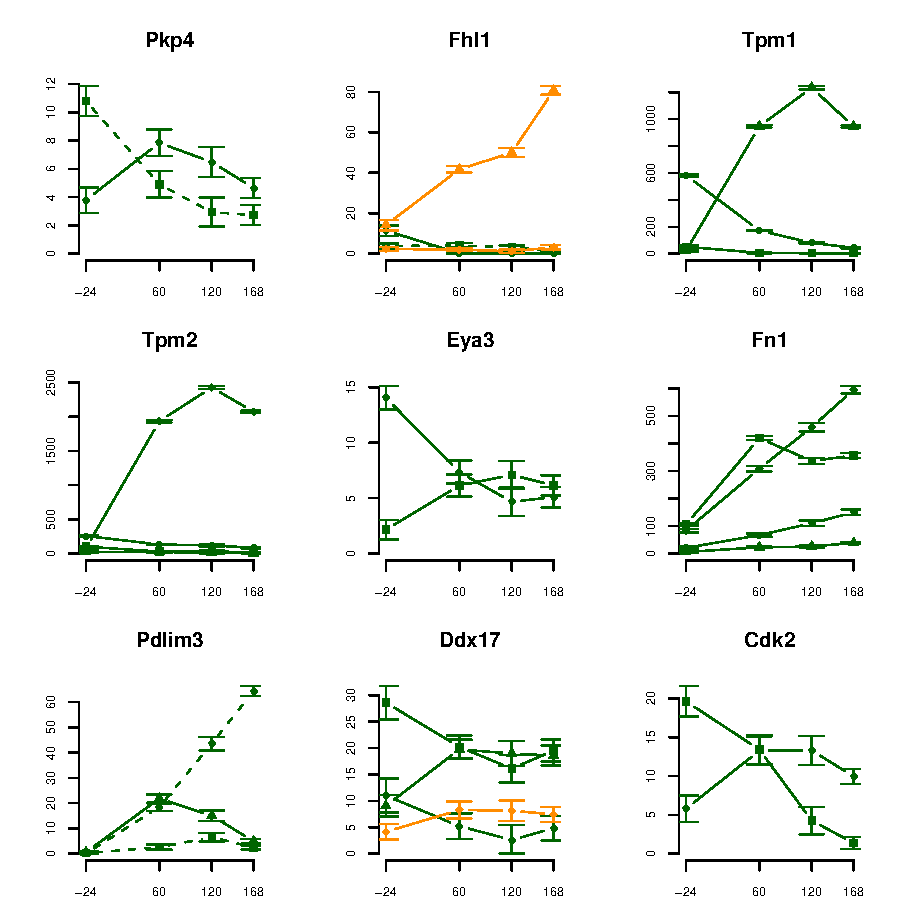
\includegraphics{pdfs/splice_overloaded}
    \caption[Selected genes with post-transcriptional
    overloading]{Selected genes with post-transcriptional
      overloading. Trajectories indicate the expression of individual
      isoforms in FPKM ($y$ axis) over time in hours ($x$
      axis). Dashed isoforms have not been previously
      annotated. Isoform trajectories are colored by TSS, so isoforms
      with the same color presumably share a common promoter and are
      processed from the same primary transcript. It is evident that
      total gene expression may remain constant during isoforms
      switching (Eya3) while in other cases changes in relative
      abundance are accompanied by changes in absolute expression. 
The Jensen-Shannon metric generalizes the notion of ``isoform
switching'' and is useful in cases with multiple isoforms
(e.g. Ddx17).    
  \label{splice_overloaded}}
\end{figure}

\begin{figure}[!ht] 
    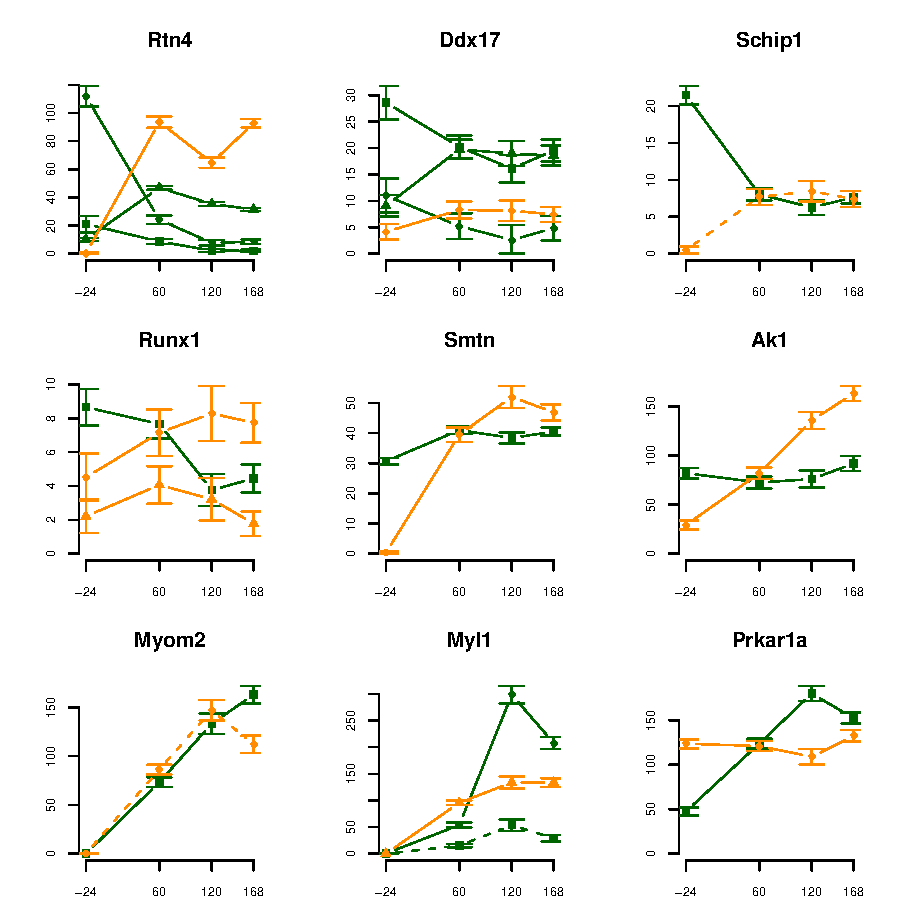
\includegraphics{pdfs/promoter_overloaded}
    \caption[Selected genes with transcriptional overloading]{Selected
      genes with transcriptional overloading. Trajectories indicate
      the expression of individual isoforms in FPKM (y axis) over time
      in hours (x axis). Dashed isoforms have not been previously
      annotated. Isoform trajectories are colored by TSS, so that
      isoforms with different colors presumably vary in their promoter
      and are processed from different primary transcripts.  \label{promoter_overloaded}}
\end{figure}

We can visualize overloading and expression dynamics with a plot that
superimposes transcriptional and post-transcriptional overloading and
gene-level expression over the time course. We refer to these as
``Minard plots'', after Charles Joseph Minard's famous depiction
of the advance and retreat of
Napoleon's armies in the campaign against Russia in 1812
\cite{Tufte2001}. Minard made use of multiple visual cues to display
numerous varying quantities in one diagram. An example of a Minard
plot for the gene
Myc is shown in Figure 3c, and others are given in Appendix B. The dotted line indicates gene-level FPKM, with measured
FPKM indicated by black circles. Grey circles indicate the arithmetic mean of
gene-level FPKM between consecutive measured time points, interpolating FPKM
at intermediate time points. The total gene expression overloading is
visualized as a swatch centered around the interpolated expression curve.
The width of the swatch encodes the amount of expression overloading between
successive time points. The color of the swatch indicates the relative
contributions of transcriptional and post-transcriptional expression
overloading.

Some genes, such as tropomyosin I and II, feature a single primary
transcript, and so all overloading is by definition post-transcriptional.
Others, like Fhl3, have two primary transcripts, but only a single isoform
arises from each, so all overloading is transcriptional. Genes with multiple
primary transcripts, one or more of which are alternatively spliced, such as
Myc or RTN4, display both forms.


\subsection{The {\tt Cufflinks} software}

The transcript assembly and abundance estimation algorithms are implemented in
freely available open source software called {\tt Cufflinks} that is available
from \newline {\tt http://cufflinks.cbcb.umd.edu/} \newline Furthermore
methods for comparing annotations across time points, and for performing the
differential expression, promoter usage and splicing tests are implemented in
the companion programs {\tt Cuffdiff} and {\tt Cuffcompare}. Instructions on
how to install and run the software are provided on the website.

The input to {\tt Cufflinks} consists of fragment alignments in the SAM format
\cite{Li2009a}. These may consist of either single fragment alignments, or alignments of mate-pairs (paired-end reads produce better assemblies and more accurate abundance estimates than single reads). {\tt Cufflinks} will assemble the transcripts using the
algorithm in Section \ref{sec:assembly}, and transcript abundances will be
estimated using the model in Section \ref{sec:abundances}. Transcript
coordinates and abundances are reported in the Gene Transfer Format (GTF).
User supplied annotations may be provided to {\tt Cufflinks} (optional input) in
which case they form the basis for the transcript abundance estimation.

Some of the algorithms here rely on sufficient depth of sequencing in order to
produce reliable output. {\tt Cufflinks} determines that depth is sufficient where
possible to check that required assumptions hold. For example, in loci where one
or more isoforms have extremely low relative expression, the observed Fisher
Information Matrix may not be positive definite after rounding errors. In this
case, it is not possible to produce a reliable variance-covariance matrix for
isoform fragment abundances. {\tt Cufflinks} will report a numerical
exception in this and similar cases. When an exception is reported, the
confidence intervals for the isoforms' abundances will be set from 0
FPKM to the FPKM for the whole gene. If such an exception is generated during
a {\tt Cuffdiff} run, no differential analysis involving the problematic
sample will be performed on that locus. 
\newpage 
\section{Appendix A: Lemmas and Theorems}

The following elementary/classical results are required for our methods and we include them so that the supplement is self-contained.

\begin{lemma}
\label{lemma:varsum}
Let $X_1,\ldots,X_n$ be random variables and $a_1,\ldots,a_n$ real numbers with $Y=\sum_{i=1}^na_iX_i$. Then
\begin{equation}
Var[Y] = \sum_{i=1}^n a_i^2Var[X_i]+2\sum_{i<j} a_ia_j Cov[X_i,X_j].
\end{equation}
\end{lemma}
\begin{lemma}[Taylor Series]
If $X$ and $Y$ are random variables then
\begin{eqnarray}
  Var[f(X,Y)] & \approx & \left(\frac{\partial f}{\partial X}(E[X],E[Y])\right)^2Var[X] \nonumber \\ & &+2\frac{\partial f}{\partial X}(E[X],E[Y])\frac{\partial f}{\partial Y}(E[X],E[Y])Cov[X,Y] \nonumber \\ & & +\left( \frac{\partial f}{\partial Y}(E[X],E[Y])\right)^2 Var[Y].
\end{eqnarray}
\end{lemma}
\begin{cor}
If $X$ and $Y$ are independent then
\begin{eqnarray}
  Var\left[log\left(\frac{X}{Y}\right)\right] & \approx & \frac{V[X]}{E[X]^2} + \frac{V[Y]}{E[Y]^2}.
\end{eqnarray}
\end{cor}
\begin{cor}
\label{lemma:varproduct}
If $X$ and $Y$ are independent random variables then
\begin{equation}
Var[XY] = Var[X]Var[Y]+E[X]^2Var[Y]+E[Y]^2Var[X].
\end{equation}
\end{cor}

The above result is exact using the 2nd order Taylor expansion (higher
derivatives vanish).

\begin{lemma}[\cite{Li2009b}]
\label{lemma:readstoprobs}
Let $a_1,\ldots,a_n,w_1,\ldots,w_n$ be real numbers satisfying: $w_i \neq 0$ and $0 \leq a_i \leq 1$ for all $i$, $\sum_{i=1}^n a_i = 1$ and $\sum_{i=1}^na_iw_i \neq 0$.  Let 
$ b_j = \frac{a_jw_j}{\sum_{i=1}^n a_iw_i}$. Then $a_j = \frac{b_j\frac{1}{w_j}}{\sum_{i=1}^n b_i\frac{1}{w_i}}$.
\end{lemma}
{\bf Proof}: \begin{eqnarray}
b_j & =  & \frac{a_jw_j}{\sum_{i=1}^n a_iw_i} \\
\Rightarrow \,  \sum_{k=1}^n \frac{b_k}{w_k} & = &   \sum_{k=1}^n \frac{a_k}{\sum_{i=1}^na_iw_i}\\
&  = &  \frac{1}{\sum_{i=1}^n a_iw_i}\\
& = & \frac{b_j}{a_jw_j}\\
 \Rightarrow \,  a_j  & =  & \frac{b_j\frac{1}{w_j}}{\sum_{i=1}^n b_i \frac{1}{w_i}}.
\end{eqnarray} \qed
\begin{prop}[\cite{ASCB2005}]
\label{prop:linearmodel}
Let $f_i(\theta) = \sum_{j=1}^d a_{ij}\theta_j + b_i$ ($1 \leq i \leq
m$) describe a linear statistical model with $a_{ij} \geq$ for all
$i,j$.  That is, $\sum_{i=1}^m f_i(\theta) = 1$. If $u_i \geq 0$ for
all $i$ then the log likelihood function
\begin{equation}
l(\theta) = \sum_{i=1}^m u_i log(f_i(\theta))
\end{equation}
is concave.
\end{prop}
{\bf Proof}: It is easy to see that 
\begin{equation}
\left( \frac{\partial^2 l}{\partial \theta_j \partial \theta_k}  \right)  = -A^Tdiag\left( \frac{u_1}{f_1(\theta)^2},\ldots,\frac{u_m}{f_m(\theta)^2}\right) A,
\end{equation}
where $A$ is the $m \times d$ matrix whose entry in row $i$ and column
$j$ equals $a_{ij}$. Therefore the Hessian is a symmetric matrix with
non-positive eigenvalues, and is therefore negative semi-definite.
\qed

\begin{defn}
\label{def:po}
A partially ordered set is a set $S$ with a binary relation $\leq$
satisfying:
\begin{enumerate}
\item $x \leq x$ for all $x \in S$,
\item If $x \leq y$ and $y \leq z$ then $x \leq z$,
\item If $x \leq y$ and $y \leq x$ then $x=y$.
\end{enumerate}
A {\em chain} is a set of elements in $C \subseteq S$ such that for every
$x,y \in C$ either $x \leq y$ or $y \leq x$. An {\em antichain} is a set of
elements that are pairwise incompatible.
\end{defn}
Partially ordered sets are equivalent to directed acyclic graphs (DAGs). The following min-max theorems relate chain partitions to antichains and are special cases of linear-programming duality. More details and complete proofs can be found in \cite{Lovasz2009}.

\begin{thm}[Dilworth's theorem]
\label{thm:Dilworth}
Let $P$ be a finite partially ordered set. The maximum number of elements in any antichain of $P$ equals the minimum number of chains in any partition of $P$ into chains.
\end{thm}
\begin{thm}[K\"{o}nig's theorem]
\label{thm:konig}
In a bipartite graph, the number of edges in a maximum matching equals
the number of vertices in a minimum vertex cover.
\end{thm}
\begin{thm}
\label{thm:dilko}
Dilworth's theorem is equivalent to K\"{o}nig's theorem.
\end{thm}
{\bf Proof}: We first show that Dilworth's theorem follows from
K\"{o}nig's theorem. Let $P$ be a partially ordered set with $n$
elements. We define a bipartite graph $G=(U,V,E)$ where
$U=V=P$, i.e. each partition in the bipartite graph is equally to
$P$. Two nodes $u,v$ form an edge $(u,v) \in E$ in the graph $G$ iff
$u<v$ in $P$. By K\"{o}nig's theorem there exist both a matching $M$ and a
a vertex cover $C$ in $G$ of the same cardinality. Let $T \subset
S$ be the set of elements not contained in $C$. Note that $T$ is an
antichain in $P$. We now form a partition $W$ of $P$ into chains by declaring $u$ and
$v$ to be in the same chain whenever there is an edge $(u,v) \in
M$. Since $C$ and $M$ have the same size, it follows that $T$ and $W$
have the same size.

To deduce K\"{o}nig's theorem from Dilworth's theorem, we begin with a
bipartite graph $G=(U,V,E)$ and form a partial order $P$ on the
vertices of $G$ by defining $u<v$ when $u \in U, v \in V$ and $(u,v)
\in E$. By Dilworth's theorem, there exists an antichain of $P$ and a
partition into chains of the same size. The non-trivial chains in $P$
form a matching in the graph. Similarly, the complement of the
vertices corresponding to the anti-chain in $P$ is a vertex cover of
$G$ with the same cardinality as the matching.  \qed

\begin{figure}[!ht] 
    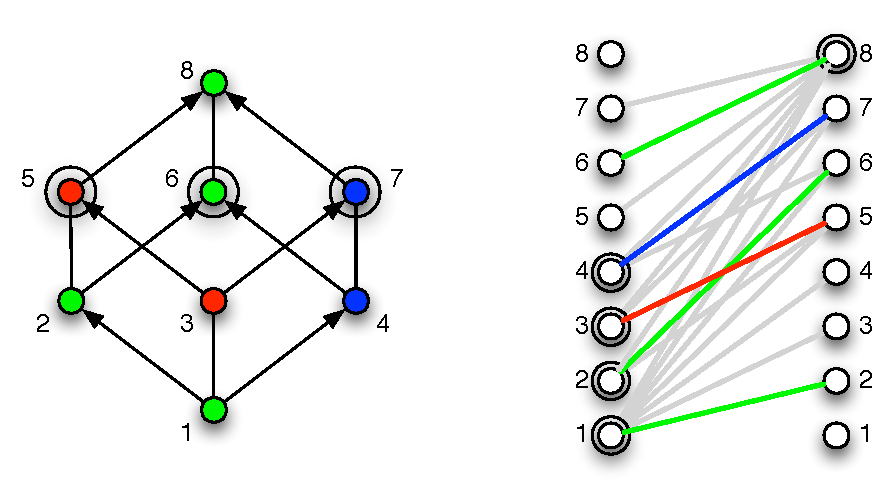
\includegraphics[scale=0.8]{pdfs/Dilworth_Konig}

%\caption[Equivalence of Dilworth's and K\"{o}nig's theorems]{
\end{figure}
The equivalence of Dilworth's and K\"{o}nig's theorems is depicted above. The
      partially ordered set with 8 elements on the left is partitioned into 3
      chains. This is the size of a minimum partition into chains, and
    is equal to the maximum size of an antichain (Dilworth's
    theorem). The antichain is shown with double circles. On the
    right, the reachability graph constructed from the partially
    ordered set on the left is shown. The maximum matching
    corresponding to the chain partition consists of 5 edges and is equal in size to the
    number of vertices in a minimum vertex cover (K\"{o}nig's
    theorem). The vertex cover is shown with double circles. Note that
    8=3+5.


\newpage
\bibliographystyle{amsplain}
\bibliography{cufflinks}
\end{document}

% long read length is required for uniquely determining genomic origin of fragments, but its fragment length that is critical for assignment of fragments to transcripts.
% The length of a set of transcripts depends on their abundances
% single read sequencing prevents the correct normalization for fragment sizes in the length.
